\documentclass{article}
\usepackage{graphicx}
\usepackage{tikz}
\usetikzlibrary{arrows.meta}
\usetikzlibrary{positioning}
\usetikzlibrary{shapes.geometric}
\usetikzlibrary{shapes.misc}


\begin{document}
\section{Expert$\rightarrow$UCD}
Alternatywa do UCD Modeller - tworzenie na podstawie opisu tekstowego.

\begin{figure}[h]
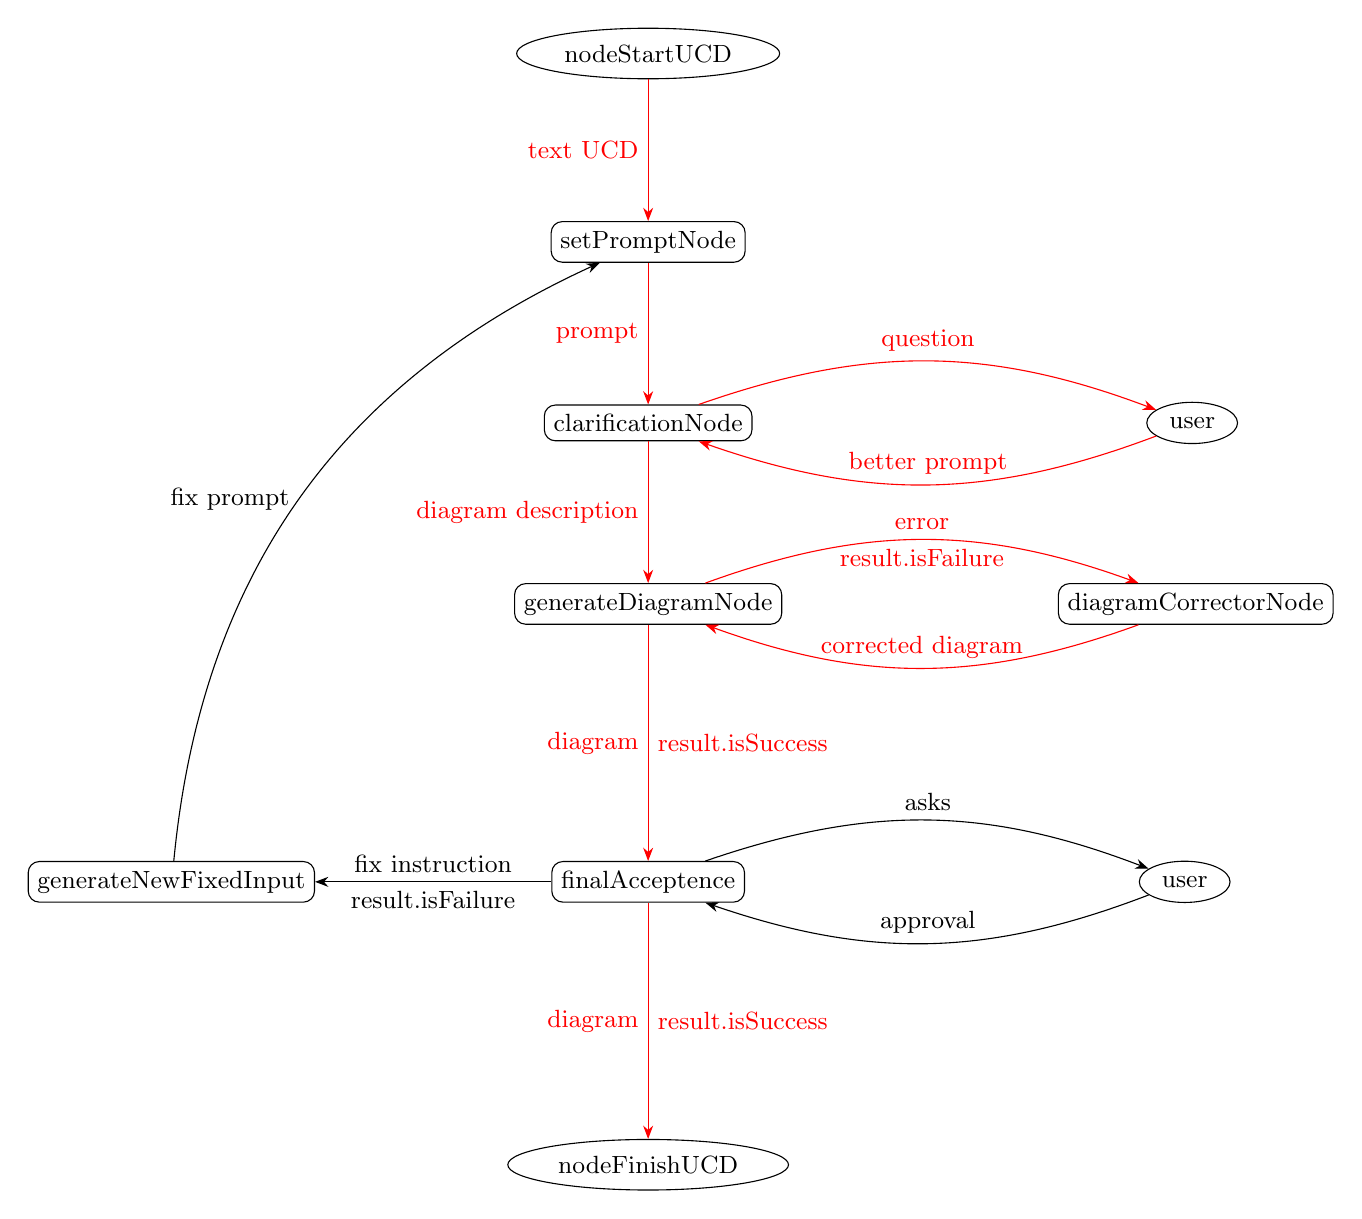
\begin{tikzpicture}[
    node distance=1.8cm and 2.5cm,
    >=Stealth,
    every node/.style={font=\small},
    process/.style={rectangle, draw, rounded corners, align=center},
    startstop/.style={ellipse, draw, align=center},
    decision/.style={diamond, draw, aspect=2, align=center}
]

% Nodes
\node[startstop] (start) {nodeStartUCD};
\node[process, below=of start] (prompt) {setPromptNode};
\node[process, below=of prompt] (clarify) {clarificationNode};
\node[startstop, right=5cm of clarify] (user) {user};
\node[process, below=of clarify] (generate) {generateDiagramNode};
\node[process, right=3.5cm of generate] (correct) {diagramCorrectorNode};
\node[process, below=3cm of generate] (accept) {finalAcceptence};
\node[startstop, below=3cm of accept] (finish) {nodeFinishUCD};
\node[startstop, right=5cm of accept] (user2) {user};
\node[process, left=3cm of accept] (newInput) {generateNewFixedInput};

% Edges
\draw[->, color=red] (start) --  node[left]{text UCD}(prompt);
\draw[->, color=red] (prompt) --  node[left]{prompt}(clarify);
\draw[->, color=red] (clarify) --  node[left]{diagram description} (generate);
\draw[->, color=red] (generate) to[bend left=20] node[below] {result.isFailure} node[above] {error} (correct);
\draw[->, color=red] (correct) to[bend left=20] node[above] {corrected diagram} (generate);
\draw[->, color=red] (clarify) to[bend left=20] node[above] {question} (user);
\draw[->, color=red] (user) to[bend left=20] node[above] {better prompt} (clarify);
\draw[->, color=red] (generate) -- node[right]{result.isSuccess} node[left]{diagram}(accept);
\draw[->, color=red] (accept) -- node[left]{diagram} node[right]{result.isSuccess} (finish);
\draw[->] (accept) to[bend left=20] node[above] {asks} (user2);
\draw[->] (user2) to[bend left=20] node[above] {approval} (accept);
\draw[->] (accept) -- node[below]{result.isFailure} node[above]{fix instruction}(newInput);
\draw[->] (newInput) to[bend left=30] node[left] {fix prompt} (prompt);



\end{tikzpicture}
\end{figure}

Rola Agent-Managera zastąpiona została przez strategię definiowaną przez przepływy miedzy etapami - graf. Rolę Agent-Evaluator pełni użytkownik (możliwa prosta podmianka - jedyny problem to ograniczenie liczby iteracji). Dla wyniku algorytmu możliwa jest wizualizacja obrazu png.

\section{UCD$\rightarrow$Scenarios}

\begin{figure}[h]
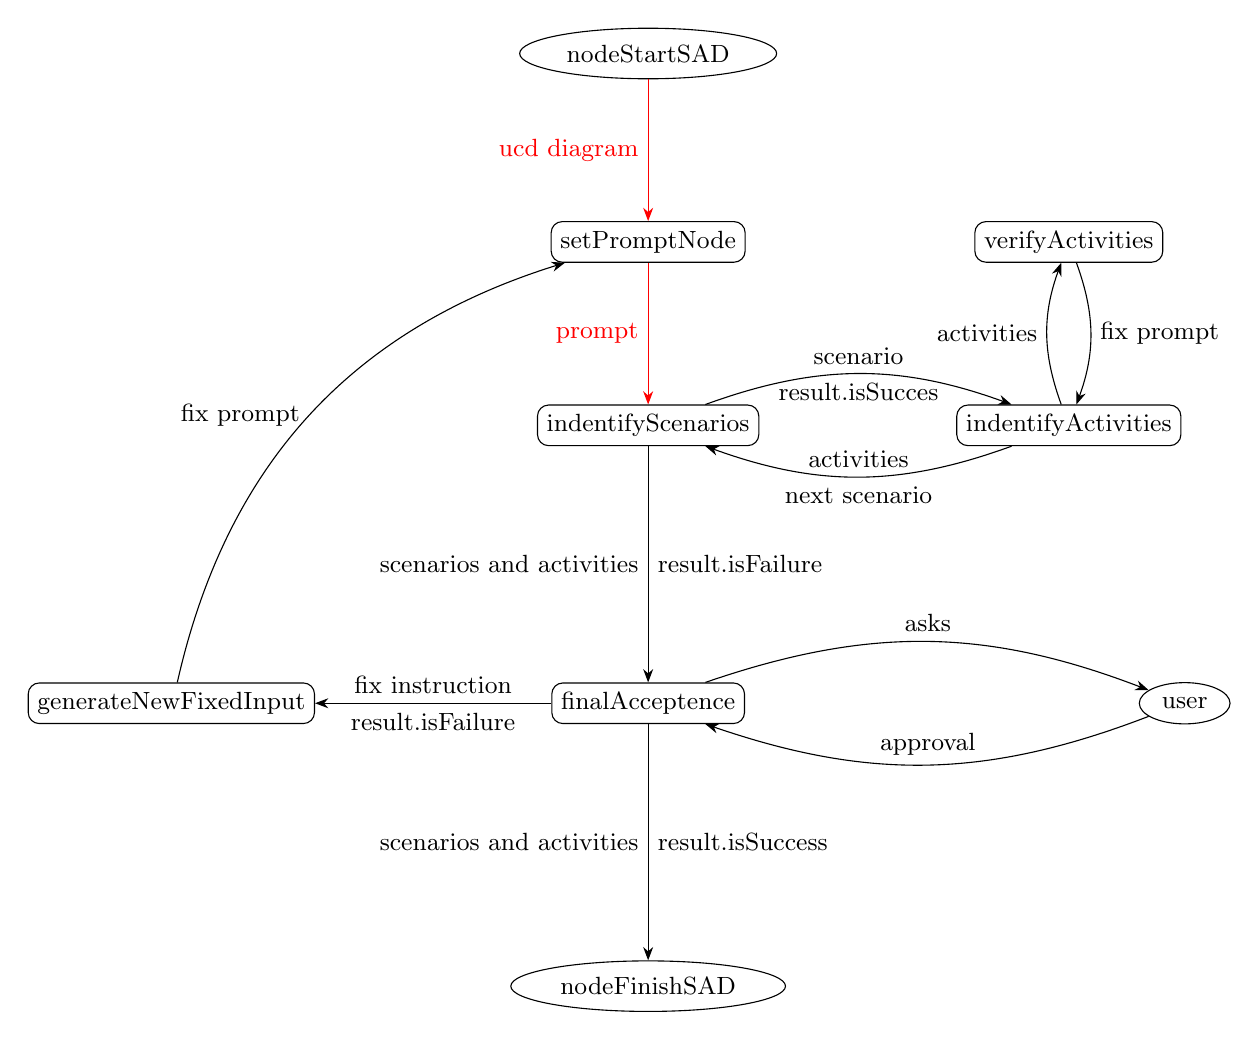
\begin{tikzpicture}[
    node distance=1.8cm and 2.5cm,
    >=Stealth,
    every node/.style={font=\small},
    process/.style={rectangle, draw, rounded corners, align=center},
    startstop/.style={ellipse, draw, align=center},
    decision/.style={diamond, draw, aspect=2, align=center}
]

% Nodes
\node[startstop] (start) {nodeStartSAD};
\node[process, below=of start] (prompt) {setPromptNode};
\node[process, below=of prompt] (ident) {indentifyScenarios};
\node[process, right=of ident] (analyze) {indentifyActivities};
\node[process, above=of analyze] (check) {verifyActivities};
\node[process, below=3cm of ident] (accept) {finalAcceptence};
\node[startstop, right=5cm of accept] (user2) {user};
\node[process, left=3cm of accept] (newInput) {generateNewFixedInput};
\node[startstop, below=3cm of accept] (finish) {nodeFinishSAD};

% Edges
\draw[->, color=red] (start) --  node[left]{ucd diagram}(prompt);
\draw[->, color=red] (prompt) --  node[left]{prompt}(ident);
\draw[->] (ident) to[bend left=20]  node[above]{scenario} node[below]{result.isSucces}(analyze);
\draw[->] (analyze) to[bend left=20]  node[left]{activities} (check);
\draw[->] (check) to[bend left=20]  node[right]{fix prompt} (analyze);
\draw[->] (analyze) to[bend left=20]  node[above]{activities} node[below]{next scenario}(ident);
\draw[->] (ident) -- node[right]{result.isFailure} node[left]{scenarios and activities}(accept);
\draw[->] (accept) to[bend left=20] node[above] {asks} (user2);
\draw[->] (user2) to[bend left=20] node[above] {approval} (accept);
\draw[->] (accept) -- node[left]{scenarios and activities} node[right]{result.isSuccess} (finish);
\draw[->] (accept) -- node[below]{result.isFailure} node[above]{fix instruction}(newInput);
\draw[->] (newInput) to[bend left=30] node[left] {fix prompt} (prompt);

\end{tikzpicture}
\end{figure}

\newpage
\section{Main}
\begin{figure}[h]
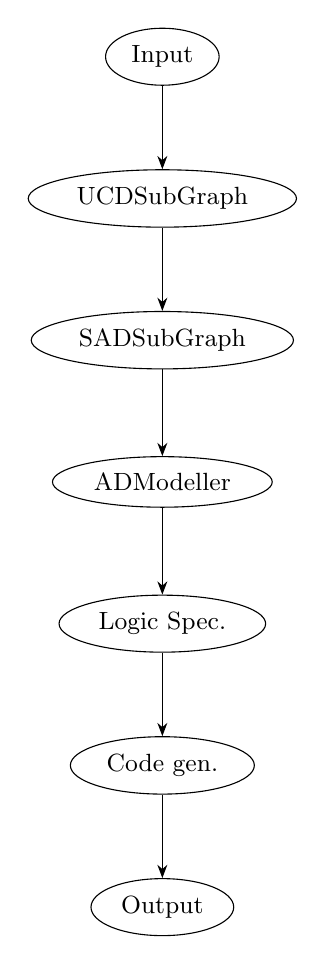
\begin{tikzpicture}[
    node distance=1.8cm and 2.5cm,
    >=Stealth,
    every node/.style={font=\small},
    process/.style={rectangle, draw, rounded corners, align=center},
    startstop/.style={ellipse, draw, align=center},
    decision/.style={diamond, draw, aspect=2, align=center}
]

% Nodes
\node[startstop] (inp) {Input};
\node[startstop, below of=inp] (ucd) {UCDSubGraph};
\node[startstop, below of=ucd] (sad) {SADSubGraph};
\node[startstop, below of=sad] (ad) {ADModeller};
\node[startstop, below of=ad] (lr) {Logic Spec.};
\node[startstop, below of=lr] (gen) {Code gen.};
\node[startstop, below of=gen] (code) {Output};

% Edges
\draw[->] (inp) -- (ucd);
\draw[->] (ucd) -- (sad);
\draw[->] (sad) -- (ad);
\draw[->] (ad) -- (lr);
\draw[->] (lr) -- (gen);
\draw[->] (gen) -- (code);

\end{tikzpicture}
\end{figure}

Uzupełnienie do poprzedniego pytania. W proponowanym rozwiązaniu User zatwierdza 'jakość' w każdym kroku na grafie Main. Czy należy rozważyć konieczność powrotu do kroków związanych z LLM (2,3,4) po krokach deterministycznych (5,6)? - Ex. kryteria jakości kodu, zmiana zdania etc.


\end{document}
